\begin{exercice*}
    Pour chaque triangle : 
    \begin{itemize}
        \item préciser le sommet de l'angle droit
        \item indiquer l'hypoténuse
        \item compléter la relation de Pythagore
    \end{itemize}
    \begin{multicols}{2}
        \begin{enumerate}
            \item 
            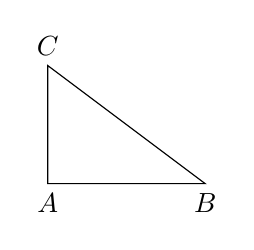
\begin{tikzpicture}[baseline={([yshift={-\ht\strutbox}]current bounding box.north)}, execute at end picture={baseline=(current bounding box.east)},scale=0.5]
                \coordinate[label=below:$A$] (A) at (1,1);
                \coordinate[label=below:$B$] (B) at (5,1);
                \coordinate[label=above:$C$] (C) at (1,4);
                \draw (A)--(B)--(C)--cycle;
                \tkzMarkRightAngles[size=0.3](B,A,C);
            \end{tikzpicture}

            $BC^2=\ldots$
            \item 
            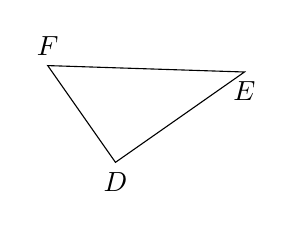
\begin{tikzpicture}[baseline={([yshift={-\ht\strutbox}]current bounding box.north)}, execute at end picture={baseline=(current bounding box.east)},scale=0.5,rotate=35]
                \coordinate[label=below:$D$] (D) at (1,1);
                \coordinate[label=below:$E$] (E) at (5,1);
                \coordinate[label=above:$F$] (F) at (1,4);
                \draw (D)--(E)--(F)--cycle;
                \tkzMarkRightAngles[size=0.3](E,D,F);
            \end{tikzpicture}

            $DE^2=\ldots$
        \end{enumerate}
    \end{multicols}
    \hrefMathalea{https://coopmaths.fr/mathalea.html?ex=4G20-1,s=2,s2=3,n=3,video=M9sceJ8gzNc,i=0&v=l}
\end{exercice*}
\begin{corrige}
    %\setcounter{partie}{0} % Pour s'assurer que le compteur de \partie est à zéro dans les corrigés
    % \phantom{rrr}
    Pour chaque triangle : 
    \begin{itemize}
        \item préciser le sommet de l'angle droit
        \item indiquer l'hypoténuse
        \item compléter la relation de Pythagore
    \end{itemize}

    \begin{enumerate}
        \item 
        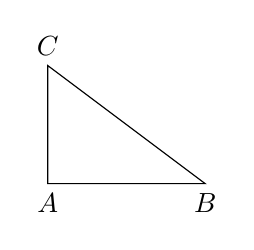
\begin{tikzpicture}[baseline={([yshift={-\ht\strutbox}]current bounding box.north)}, execute at end picture={baseline=(current bounding box.east)},scale=0.5]
            \coordinate[label=below:$A$] (A) at (1,1);
            \coordinate[label=below:$B$] (B) at (5,1);
            \coordinate[label=above:$C$] (C) at (1,4);
            \draw (A)--(B)--(C)--cycle;
            \tkzMarkRightAngles[size=0.3](B,A,C);
        \end{tikzpicture}

        $BC^2=\ldots$\\
        {\red $A$ est le sommet de l'angle droit.\\$[BC]$ est l'hypoténuse.\\$BC^2=BA^2+AC^2$}
        \item 
        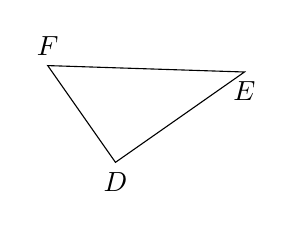
\begin{tikzpicture}[baseline={([yshift={-\ht\strutbox}]current bounding box.north)}, execute at end picture={baseline=(current bounding box.east)},scale=0.5,rotate=35]
            \coordinate[label=below:$D$] (D) at (1,1);
            \coordinate[label=below:$E$] (E) at (5,1);
            \coordinate[label=above:$F$] (F) at (1,4);
            \draw (D)--(E)--(F)--cycle;
            \tkzMarkRightAngles[size=0.3](E,D,F);
        \end{tikzpicture}

        $DE^2=\ldots$\\
        {\red $D$ est le sommet de l'angle droit.\\$[EF]$ est l'hypoténuse.\\$DE^2=EF^2-DF^2$}
    \end{enumerate}
\end{corrige}

